\documentclass{beamer}

% Use metropolis theme
\usetheme[progressbar=frametitle]{metropolis}
\usepackage{minted}
\usepackage{hyperref}

\title{How to Use Python and Mathematical Modeling to Better Understand the Impact of Electricity Pricing on Consumption}

\date{November 2, 2023}
\author{Saba Nejad}
\institute{PyData NYC 2023}

\begin{document}
\maketitle

\section{Outline}

\begin{frame}{Overview of the Talk}
  \begin{itemize}
  \item Introduce the problem space; defining terminology
  \item Introduce the trial and the dataset
  \item Mathematical Model
  \item Data prep, cleaning, processing
  \item Results
  \end{itemize}
\end{frame}

\section{Introducing the Problem Space}

\begin{frame}{The Power Grid}
  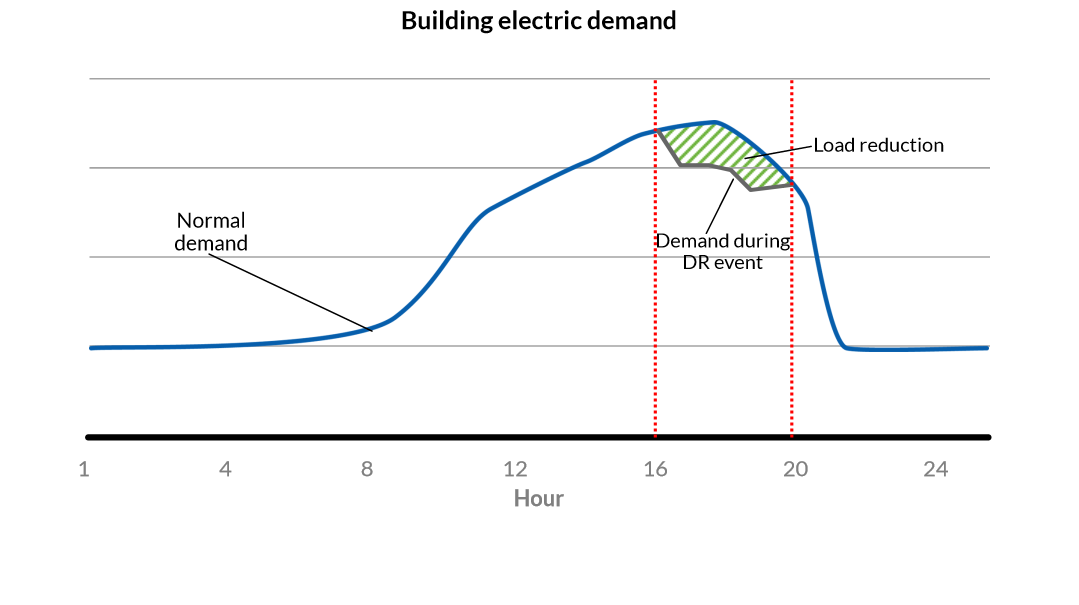
\includegraphics[width=1.00\textwidth]{images/demand-response.png}
\end{frame}

\begin{frame}{The Power Grid}
  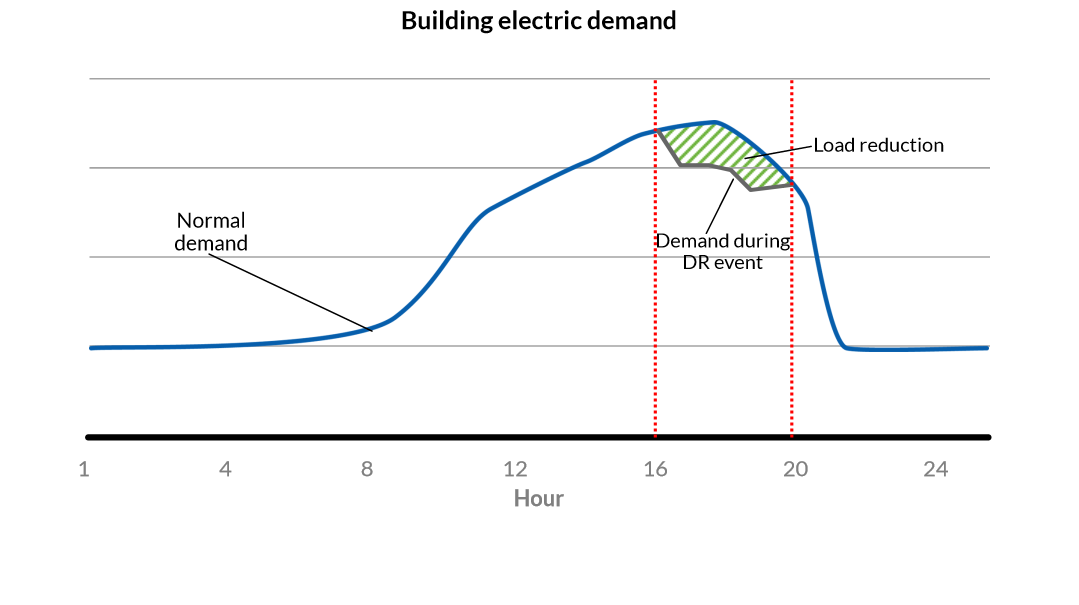
\includegraphics[width=1.00\textwidth]{images/demand-response.png}
  \begin{itemize}
  \item[]<+-> system operators: resposible for reliable delivery of electricity to consumers
  \item[]<+-> demand response: 
  \item[]<+-> time of use pricing:
  \item[]<+-> dynamic time of use pricing:
  \end{itemize}
\end{frame}

\begin{frame}{Mathematical Model}
  \begin{enumerate}
    \item fundamental problem of causal analysis
    \item close enough to random sample: minimum wage problem, NJ and east PA, cite paper
    \url{https://davidcard.berkeley.edu/papers/njmin-aer.pdf}
  \end{enumerate}
\end{frame}

\begin{frame}{Low Carbon London Smart Meter Trial}
  \begin{itemize}
    \item[]<+-> motivation and experiment design
    \item[]<+-> shortfalls
    \url{https://data.london.gov.uk/dataset/smartmeter-energy-use-data-in-london-households}
  \end{itemize}
\end{frame}

\begin{frame}{What did we learn?}
  \begin{itemize}
    \item[]<+-> a little bit about electricity marketsssss
    \item[]<+-> causal analysis
    \item[]<+-> break down your data to match the mathematical model at hand
    \item[]<+-> how was the data aggregated? is there bias? how does that impact your analysis and results?
  \end{itemize}
\end{frame}

\begin{frame}{Thank You}
  \begin{itemize}
  \item \url{https://github.com/sabanejad}
  \item \url{https://www.linkedin.com/in/sabanejad/}
  \end{itemize}
\end{frame}

\end{document}